\paragraph{Proposition 2.28} Låt $\bm{u}$, $\bm{v}$, $\bm{w}$ vara kolumnvektorer i rummet och låt $A=\begin{pmatrix}\bm{u}\\\bm{v}\\\bm{w}\end{pmatrix}$
Då är $det(A)=(\bm{u}\times \bm{v})\cdot \bm{w}$.

\paragraph{Sats 2.29} Låt $A=\begin{pmatrix}\bm{u}\\\bm{v}\\\bm{w}\end{pmatrix}$ där $\bm{u}$, $\bm{v}$, $\bm{w}$ är kolumnvektorer i rummet
och låt $V$ vara volymen av parallellepipeden som spänns av $\bm{u}$, $\bm{v}$, $\bm{w}$.\\
Då är $det(A)=\bigg\{ \begin{matrix}
    V\text{ om $\bm{u}$, $\bm{v}$, $\bm{w}$ högerorienterat}\\
    -V\text{ om $\bm{u}$, $\bm{v}$, $\bm{w}$ vänterorienterat}
\end{matrix}$\\
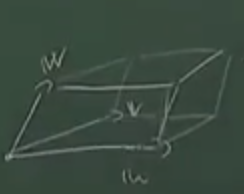
\includegraphics[scale=0.5]{imgs/22-02-07img01.png}

\paragraph{Ex} Låt $\bm{u}=\begin{pmatrix}1\\0\\2\end{pmatrix}$, $\bm{v}=\begin{pmatrix}2\\3\\1\end{pmatrix}$, $\bm{w}=\begin{pmatrix}2\\1\\1\end{pmatrix}$.
Avgör om $(\bm{u},\bm{v},\bm{w})$ är högerorienterat.
\subparagraph{Lösning} 
\begin{equation*}
    det(\bm{u},\bm{v},\bm{w})=
    \begin{vmatrix}1&2&2\\0&3&1\\2&1&1\end{vmatrix}
    =1\cdot (3\cdot 1- 1\cdot 1)-2(0\cdot 1-2\cdot 1)+2(0\cdot 1-2\cdot 3)
    =2+4-12=-6
\end{equation*}
Determinanten är negativ, alltså är $(\bm{u},\bm{v},\bm{w})$ vänsterorienterat.

\paragraph{Proposition 2.31} Låt $\bm{u}$, $\bm{v}$, $\bm{w}$, $\bm{w}_{1}$, $\bm{w}_{2}$ vara vektorer i rummet.
\begin{enumerate}
    \item 
        $\begin{vmatrix}
            \vline&\vline&\vline\\
            e_{x}&e_{y}&e_{z}\\
            \vline&\vline&\vline
        \end{vmatrix} = 
        \begin{vmatrix}
            1&0&0\\
            0&1&0\\
            0&0&1
        \end{vmatrix}=1$

    \item 
        $\begin{vmatrix}
            c\bm{u}&\bm{v}&\bm{w}
        \end{vmatrix}=c\begin{vmatrix}
            \bm{u}&\bm{v}&\bm{w}
        \end{vmatrix}$

    \item 
        $\begin{vmatrix}
            \bm{u}&\bm{v}&\bm{w}
        \end{vmatrix}=
        -\begin{vmatrix}
            \bm{v}&\bm{u}&\bm{w}
        \end{vmatrix}=
        -\begin{vmatrix}
            \bm{w}&\bm{v}&\bm{u}
        \end{vmatrix}$

    \item 
        $\begin{vmatrix}
            \bm{u}&\bm{v}&\bm{w}_{1}+\bm{w}_{2}
        \end{vmatrix}=
        \begin{vmatrix}
            \bm{u}&\bm{v}&\bm{w}_{1}
        \end{vmatrix}+
        \begin{vmatrix}
            \bm{u}&\bm{v}&\bm{w}_{2}
        \end{vmatrix}$

    \item 
        $\begin{vmatrix}
            \bm{u}&\bm{u}&\bm{v}
        \end{vmatrix}=0$
    \item $det(A^{t})=det(A)$
\end{enumerate}

\chapter{Matris Invers Avs 2.3}
\paragraph{Definition} En $n\times n$-matris $I$ kallas för en matrisidentitet om $AI=A=IA$ för alla $n\times n$-matriser $A$.
En $n\times n$-matris $B$ sägs vara en invers till $A$ om $AB=I=BA$.
\\\\
För tal är $1$ identiteten och inversen av $a\neq 0$ är $\frac{1}{a}$.\\
För $2\times 2$-matriser är $I=\begin{pmatrix}1&0\\0&1\end{pmatrix}$.\\
För $3\times 3$-matriser är $I=\begin{pmatrix}1&0&0\\0&1&0\\0&0&1\end{pmatrix}$.\\
Dessa är de enda identiteterna.\\
Om en matris $A$ har en invers då är den unik.
Vi betecknar den $A^{-1}$.

\paragraph{Sats 2.36} En $2\times 2$-matris $A=\begin{pmatrix}a&b\\c&d\end{pmatrix}$ har en invers om och endast om $det(A)\neq 0$.
Om $A$ har en invers då är den $A^{-1}=\frac{1}{det(A)}\begin{pmatrix}d&-b\\-c&a\end{pmatrix}$.
\subparagraph{Bevis} Antag att $det(A)\neq 0$. Då är
\begin{center}
    $A(\frac{1}{det(A)})\begin{pmatrix}
        d&-b\\-c&a
    \end{pmatrix}=
    \frac{1}{det(A)}\begin{pmatrix}
        a&b\\c&d
    \end{pmatrix}\begin{pmatrix}
        d&-b\\-c&a
    \end{pmatrix}=
    \frac{1}{det(A)}\begin{pmatrix}
        ad-bc&a(-b)+ba\\cd+d(-c)&c(-b)+da
    \end{pmatrix}=
    \frac{1}{det(A)}\begin{pmatrix}
        ad-bc&0\\0&ad-bc
    \end{pmatrix}=
    \frac{1}{det(A)}\begin{pmatrix}
        det(A)&0\\0&det(A)
    \end{pmatrix}=\begin{pmatrix}
        1&0\\0&1
    \end{pmatrix}$
\end{center}
Att $(\frac{1}{det(A)}\begin{pmatrix}a&-b\\-c&a\end{pmatrix})A=\begin{pmatrix}1&0\\0&1\end{pmatrix}$ visas på samma sätt.\\
Då är alltså $\frac{1}{det(A)}\begin{pmatrix}d&-b\\-c&a\end{pmatrix}$ inversen till A.
Antag att $det(A)=0$.\\
Eftersom determinanten är arean som spänns av kolumnvektorerna så är kolumnvektorerna i detta fall parallella.

$A=\begin{pmatrix}\bm{u}&k\bm{u}\end{pmatrix}$
%Vi antar, för att få en motsättning, att det finns en invers $B=\begin{pmatrix}\hline&\bm{v}^{t}&\hline\\\hline&\bm{w}^{t}&\hline\end{pmatrix}$
Då är $BA=\begin{pmatrix}
    %\hline&\bm{v}^{t} & \hline\\
    %\hline&\bm{w}^{t} & \hline
\end{pmatrix} \cdot 
\begin{pmatrix}
    \vline&\vline\\
    \bm{u}&k\bm{u}\\
    \vline&\vline
\end{pmatrix} =
\begin{pmatrix}
    \bm{v}^{t}\cdot\bm{u} & k\bm{v}^{t}\cdot \bm{u}\\
    \bm{w}^{t}\cdot \bm{u} & k\bm{w}^{t}\cdot \bm{u}
\end{pmatrix}$ 
men också 
$BA=\begin{pmatrix}1&0\\0&1\end{pmatrix}$.

Speciellt är  $\bm{w}^{t}\cdot \bm{u}=0$ men $k\bm{w}^{t}\cdot\bm{u}=1\Leftrightarrow \bm{w}^{t}\cdot \bm{u} = \frac{1}{k}$ vilket är omöjligt!
Därför finns det ingen invers! $\blacksquare$

\chapter{Geometrisk och linjära avbildningar}
\section{Linjära avbildningar}

\paragraph{Definition} Låt $V$ och $W$ vara mängder av vektorer.
En funktion $f:V\rightarrow W$ sägs vara en \underline{linjär avbildning} om \\
$f(\bm{v}_{1}+\bm{v}_{2})=f(\bm{v}_{1})+f(\bm{v}_{2}), \forall \bm{v}_{1}, \bm{v}_{2} \in V$\\
$f(c\bm{v})=c\cdot f(\bm{v}), \forall \bm{v}\in V, c\in \mathbb{R}$

\paragraph{Ex} Låt $V$ vara någon mängd av vektorer (en linje, ett plan eller ett rum) och låt $a\in\mathbb{R}$. 
Vi definierar en funktion $f:V\rightarrow V$ genom $f(\bm{v})=a\bm{v}$.
Då är $f$ linjär! Varför?
Jo:
\begin{equation*}
    f(\bm{v}_{1}+\bm{v}_{2})=a(\bm{v}_{1}+\bm{v}_{2})=a\bm{v}_{1}+a\bm{v}_{2}=f(\bm{v}_{1})+f(\bm{v}_{2})
\end{equation*}
\begin{equation*}
    f(c\bm{v})=a(c\bm{v})=(ac)\bm{v}=c(a\bm{v})=c(a\bm{v})-c\cdot f(\bm{v})
\end{equation*}

\paragraph{Ex} Låt $V=\mathbb{R}$ och $f(x)=x^{2}$.
Då är $f$ \underline{inte} linjär!
Varför? Jo:
\begin{equation*}
    f(cx)=(cx)^{2}=c^{2}x^{2}\neq cx^{2}=c\cdot f(x) \text{ så länge $c\neq 0$ och $c\neq 1$}
\end{equation*}
Alltså $f(cx)\neq cf(x)$ och därför är f inte linjär.

\paragraph{Ex} Låt $V$ vara planet eller rummet och säg att vi har fixerat ett koordinatsystem så att vektorer kan skrivas som $\bm{v}=\begin{pmatrix}
    \bm{v}_{x}\\\bm{v}_{y}\\\bm{v}_{z}
\end{pmatrix}$.
Låt $A$ vvara en matris. Då är funktionen $f:V\rightarrow V$ given av $f(\bm{v})=A\bm{v}$ av en linjär avbildning.
Varför? Jo:
\begin{equation*}
    f(\bm{v}_{1}+\bm{v_{2}})=A(\bm{v}_{1}+\bm{v}_{2})=A\bm{v}_{1}+A\bm{v}_{2}=f(\bm{v}_{1})+f(\bm{v}_{2})
\end{equation*}
\begin{equation*}
    f(c\bm{v})=A(c\bm{v})=cA\bm{v}=c\cdot f(\bm{v})
\end{equation*}

\paragraph{Ex} Om $f:V\rightarrow W$ är linjär då är $f(\bm{O})=0$.
\subparagraph{Lösning} Vi har att $f(c\bm{v})=c\cdot f(\bm{v}), \forall c\in \mathbb{R}$.
Låt $c=0$ så får $f(0\cdot \bm{v})=0f(\bm{v})\Leftrightarrow f(0)=\bm{0}$
